\section{Carrier-Grid Compression Methodology}
\label{sec:method}

\begin{figure}[t]
\centering
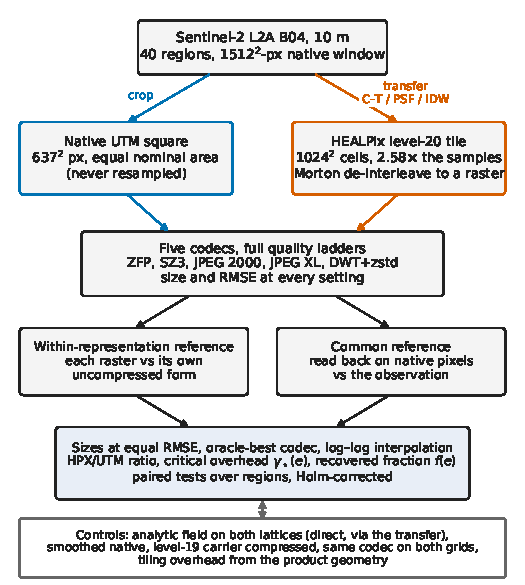
\includegraphics[width=\columnwidth]{figures/fig_workflow}
\caption{The chain the paper measures. Each native window yields an
equal-area UTM square (Section~\ref{sec:utm_crop}) and a HEALPix level-20
tile filled by a transfer (Section~\ref{sec:resampler}); both go through
the same codec sweep (Section~\ref{sec:codecs}) and are compared at equal
error under two references (Sections~\ref{sec:rd_protocol}
and~\ref{sec:common_reference}); the outcome is the size ratio and the
critical overhead of Section~\ref{sec:headline}, and the controls of
Sections~\ref{sec:support_controls}, \ref{sec:level_choice}
and~\ref{sec:same_codec} test what drives it.}
\label{fig:workflow}
\end{figure}

Fig.~\ref{fig:workflow} shows the chain from the native product to the
verdict; the subsections below describe each step.

\subsection{From a Nested Chunk to a 2-D Raster}
\label{sec:morton}
Every codec used here is a generic 2-D array or image compressor with no
knowledge of HEALPix. A chunk must therefore first become an ordinary
raster in which horizontal and vertical neighbours are spatial
neighbours. A nested chunk of $4^{\delta}$ cells (all descendants,
$\delta$ levels down, of one parent) is a 1-D array indexed by a Morton
(Z-order) code. Bit $b$ of the local $x$ coordinate sits at bit $2b$ of
the index, and bit $b$ of $y$ at bit $2b+1$. De-interleaving the bits
recovers $(x,y)$ for every cell and scatters the array into a
$2^{\delta}\times2^{\delta}$ raster, exactly invertibly. We use $\delta=10$: the $1024\times1024$ level-20 descendants
of one level-10 parent form one \term{carrier} tile, large enough to amortise
per-chunk codec overhead and small enough to stay a practical storage
unit. This reshaping is the only HEALPix-specific step; all later steps
work on a plain float32 raster. That raster still carries three marks of
its origin. The first is the kernel that filled it from the sensor grid.
The second is the shape anisotropy of equal-area HEALPix cells, a local
axis-length ratio of up to $\sim\!1.7$ between the raster axes. Both
affect compressibility (Section~\ref{sec:resampler}). The third is its
orientation. In the UTM zone of a scene its axes run at about $45^\circ$
to north (Fig.~\ref{fig:utm_crop_footprints}), so the row and column
predictors of the codecs follow diagonals of the native raster. What
that orientation costs or saves has not been measured
(Section~\ref{sec:limitations}).

\subsection{Equal-Area Native UTM Comparison}
\label{sec:utm_crop}
Both sides must cover the same nominal area, and a \term{carrier} tile
projected into the UTM zone of a scene is a rotated square. An
axis-aligned bounding box around it holds about twice the pixel count of
the true footprint and would penalise the native side. Each grid is
therefore compared in its own geometry, matched by ground area. HEALPix is equal-area, so the ground area of a level-20 tile is a
geometric constant: by \eqref{eq:healpix_width}, a $1024\times1024$-cell
tile covers a square of side $1024\,\Delta_{\mathrm{eq}}(20)\approx\SI{6.37}{km}$,
about $636.7$ native \SI{10}{m} pixels, rounded to $637$. For each scene a
$637\times637$-pixel axis-aligned square is cut from the native Sentinel-2
B04 raster. It is centred on the native pixel nearest to the mean
longitude and latitude of the tile's cells, computed with
\texttt{healpix\_geo} on the WGS84 ellipsoid~\cite{odaka2026grid4earth}.
``Equal-area'' is shorthand for equal \emph{nominal projected} area: UTM
is conformal, and rounding $636.7$ to $637$ alone adds about $0.1\%$ of
area. These terms are small next to the $2.58\times$ oversampling under
study. Both representations have a fixed
raw size across regions, \SI{1.623}{MB} for the \term{native crop}
($637^2\times\SI{4}{B}$) and \SI{4.194}{MB} for the HEALPix tile, with no
fill value on either side.

Matching by area means each grid is compressed in the frame it is stored
in, with no resampling of the native side, the comparison a practitioner
faces. It also means the two representations encode different ground
over part of their extent. Over the 40 regions the intersection is
$74$--$83\%$ of the crop ($81\%$ median), an intersection-over-union of
about $0.68$ (Fig.~\ref{fig:utm_crop_footprints}). Supports that
differ over a fifth of their extent can have different entropies.
Section~\ref{sec:support_controls} constrains the effect with an analytic
field that both geometries sample identically. That control reproduces
the decline of the measured gap to within $5$--$24\%$, and the crossover
itself once the field passes through the \term{transfer}. This makes it
unlikely that the mismatch explains the decline. It does not isolate the
mismatch's contribution to the narrow crossover at the loosest \term{target}.
The mismatch matters
more for cross-grid comparisons of reconstruction \emph{error}, which is
why the \term{common-reference} evaluation of
Section~\ref{sec:common_reference} is restricted to the intersection.

\begin{figure}[t]
\centering
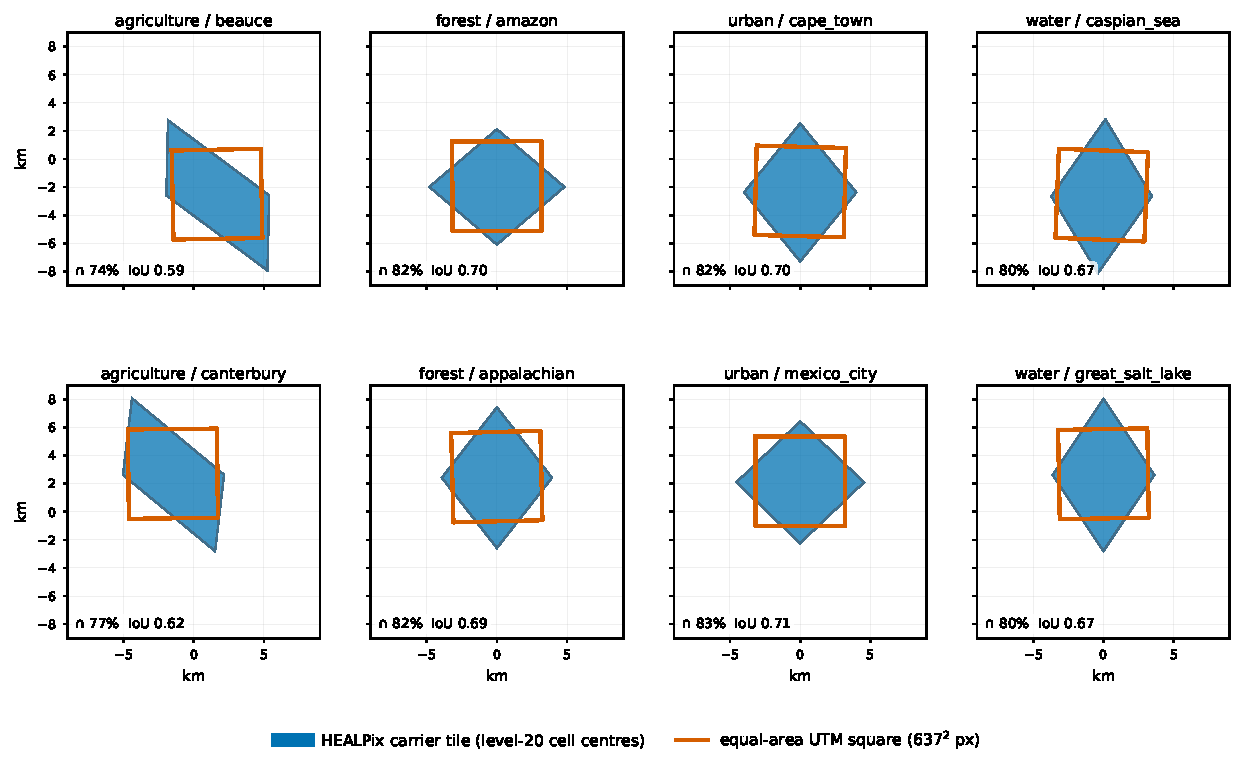
\includegraphics[width=\columnwidth]{figures/fig_utm_crop_footprints}
\caption{HEALPix tile footprint (blue, the convex hull of its level-20 cell centres) and the axis-aligned, equal-area $637\times637$ native UTM square compressed on the UTM side (red outline), for a sample of regions, in a local metric frame at a common scale. Each panel states the intersection as a fraction of the crop and the intersection over union.}
\label{fig:utm_crop_footprints}
\end{figure}

\subsection{The Resampling Kernel Is Part of the Result}
\label{sec:resampler}
Filling the level-20 tile means resampling the native raster onto the
HEALPix cell centres, a step with no counterpart on the UTM side, and the
kernel decides what the codec sees. Cell anisotropy already matters: at
fixed area the two local sample spacings scale as $\sqrt{1.7}$ and
$1/\sqrt{1.7}$, so the longer spacing comes closer to the native
\SI{10}{m} pitch than the nominal \SI{6.2}{m} scale suggests, while the
shorter one oversamples it further. The
\term{carrier} used throughout is a Clough--Tocher piecewise-cubic
interpolant~\cite{clough1965plate} over a Delaunay triangulation of the
native pixel centres. It is the \texttt{CloughTocherResampler} of the
\texttt{healpix-resample} package~\cite{delouis2026resample}, a Torch
implementation of the same construction that SciPy offers as
\texttt{griddata(method="cubic")}, close to it but not identical bit for
bit; it is distinct from the separable bicubic interpolation of a regular
raster. It brings the HEALPix spectrum close to the native one. A Shepard-type
inverse-distance average over the four nearest neighbours is kept as a
control, with a kernel width set to the HEALPix \emph{output} scale
($\sim\SI{6.2}{m}$) instead of the \SI{10}{m} \emph{input} spacing. It
leaves no excess power in the top octave ($0.92$ of the observation's).
It is, however, $2.0$ times less accurate than Clough--Tocher against an
analytic field, and its output costs about twice the bytes at equal
error (Section~\ref{sec:transfer_cost}). Kernels are compared with the
approximation-order framework of~\cite{blu1999fourier} and the kernel
comparison of~\cite{thevenaz2000interpolation}, by scoring each against
an analytic field. Section~\ref{sec:transfer_cost} rebuilds the \term{carrier}
with the PSF-aware and inverse-distance \term{transfers} and repeats the sweep
on the 40 regions. Section~\ref{sec:support_controls} scores five
kernels on the 40 regions, all of which pass the window audit of
Appendix~\ref{app:window_radiometry}. The crossover reported
below is a property of the \term{carrier} built with this \term{transfer}. The kernel
that fills a HEALPix grid from a sensor grid is a scientific choice, and
a kernel mismatched to the source sampling can change which of two grids
looks more storage-efficient once compressed.

The PSF-aware \term{transfer} is described here so that this paper stands on its
own. It models each native pixel as a Gaussian-weighted sum of the latent
field at the level-20 cell centres, with the instrument's response as the
weight (nominal B04 width \SI{12.5}{m} FWHM). It assembles that forward
operator as a sparse matrix from cells to samples. It then estimates the
cell values by damped least squares, solved by conjugate gradients on
the normal equations with a damping of $\lambda=10^{-3}$, the value at
which the companion study reports its accuracy. Its estimand is
therefore the latent field before the instrument blur. The companion
study measures that it recovers $15.4\%$ to $19.6\%$ of the blur on
noise-free fields, and Section~\ref{sec:transfer_cost} prices the bytes
this sharper estimand costs. The PSF-aware \term{transfer} comes from the
\texttt{healpix-resample} package at its tag
\texttt{jstars-submission}, the version the companion paper describes.
The environment record written with every sweep names the checkout it
ran against, because the package's PSF width convention changed once
between versions during this work.

\subsection{Codecs Compared}
\label{sec:codecs}
No custom or HEALPix-aware codec is used. We evaluate established,
independently maintained codecs, so that any redundancy that survives
compression can be exploited with tools a practitioner can already
install. Learned codecs are absent by design. They have reshaped the
rate--distortion frontier for natural images since~\cite{balle2017endtoend}
and reached remote sensing, including on-board
use~\cite{valsesia2019onboard}. Their performance, however, depends on
the training distribution, and no pair of models trained symmetrically
on the two grids exists. Compression practice for optical space imagery
is surveyed in~\cite{blanes2014tutorial}. The mission-side standards
there, the CCSDS wavelet coder and its multispectral
successor~\cite{hernandez2021ccsds123}, \term{target} the on-board bandwidth
problem, where complexity, memory and channel errors constrain the coder
as much as its rate~\cite{abrardo2010onboard}. The question here is
archive-side. Five general-purpose compressors are applied identically
on both grids:
\begin{itemize}
    \item \textbf{ZFP}~\cite{lindstrom2014zfp}: a fixed-accuracy compressed floating-point array codec based on a near-orthogonal block transform;
    \item \textbf{SZ3}~\cite{liang2022sz3}: a modular, prediction-based, error-bounded lossy compressor for scientific floating-point data;
    \item \textbf{JPEG~2000}~\cite{taubman2000jpeg2000}, lossy and lossless: a wavelet codec with embedded block coding and optimised truncation (EBCOT);
    \item \textbf{JPEG~XL}~\cite{alakuijala2019jpegxl}, lossy and lossless: a multiscale (\emph{Squeeze}) modular mode for lossless and near-lossless coding and a block-DCT (\emph{VarDCT}) mode for lossy coding;
    \item \textbf{DWT+Zstandard}: a textbook baseline, a multi-level 2-D wavelet transform~\cite{antonini1992wavelet} with uniform scalar quantisation, entropy-coded with Zstandard~\cite{rfc8878zstd}.
\end{itemize}
Each codec is swept over its own quality parameter to trace a full
rate--distortion curve: tolerance for ZFP, absolute error bound for SZ3,
quality/rate for JPEG~2000, distance/level for JPEG~XL, quantisation
depth for DWT+Zstandard. JPEG~2000 and JPEG~XL add one lossless point
each. Each ladder runs from near-lossless to settings coarse enough that
the loosest \term{target} of Section~\ref{sec:rd_protocol} is exceeded on every
region whose contrast permits it: ZFP tolerance up to $3$, SZ3 error
bound up to $1$, JPEG~2000 compression ratio up to $4000$, JPEG~XL down
to its coarsest quality level and largest Butteraugli distance,
DWT+Zstandard down to two quantisation bits. This gives 71 operating
points per region and grid. Sweeping the parameter bypasses each codec's
rate control on purpose; in JPEG~2000 that means the quality layers and
the post-compression optimisation that fills them, a research subject in
itself~\cite{auli2008scalability}. A rate controller targets a budget,
while this comparison needs an \emph{achieved} error or size on both
grids, so the matching is done afterwards
(Section~\ref{sec:rd_protocol}).

\subsection{Codec Preference Is Empirical}
\label{sec:why_quadtree}
The $2\times2$ block structure of the de-interleaved raster aligns with
HEALPix parent--child groups, and the experiments here do not isolate an
advantage from that alignment. A native UTM raster supports the same
dyadic transforms, and Section~\ref{sec:results} finds the same shift
towards JPEG~2000 and JPEG~XL at aggressive ratios on \emph{both} grids.
The codec ranking is therefore an empirical finding about these codecs on
this imagery; a direct test of a quadtree-native coder
(Appendix~\ref{app:quadtree}) found no advantage large enough to matter.
